\chapter{Progettazione}
\label{capitolo5}
\thispagestyle{empty}

\noindent Nei paragrafi successivi verranno illustrate le fasi di implementazione del gestore di dati personali, motivando le scelte implementative e le eventuali differenze che si creano rispetto a quanto detto in Analisi.

Per la realizzazione del gestore \`e stato utilizzato il linguaggio Java. https://docs.oracle.com/javase/specs/jls/se8/html/index.html http://docs.oracle.com/javase/8/docs/api/

Fra i principi generali seguiti in Progettazione troviamo l’inversione delle dipendenze, la separazione delle responsabilit\`a, il principio di sostituibilit\`a di Liskov e il gi\`a citato rasoio di Occam. Secondo il principio di inversione delle dipendenze, \`e necessario che le dipendenze presenti all’interno del codice non siano fra classi ma fra interfacce, in modo da evitare che la struttura possa risentire di cambiamenti che avvengono a basso livello. Il principio di separazione delle responsabilit\`a stabilisce che ogni classe deve avere un solo compito, da svolgere interamente, ma mai pi\`u di uno: lo sviluppo di classi con pi\`u di una responsabilit\`a genera dipendenze non volute fra le classi, rendendo il codice fragile. Infine, il principio di sostituibilit\`a di Liskov si applica ai casi di ereditariet\`a fra classi, e ne regola il rapporto: ogni sottoclasse deve poter essere utilizzata al posto della classe base senza che ci si accorga della differenza.

\section{Flusso del programma}
inserire grafico

\section{Accounting}
\begin{figure} [h]
	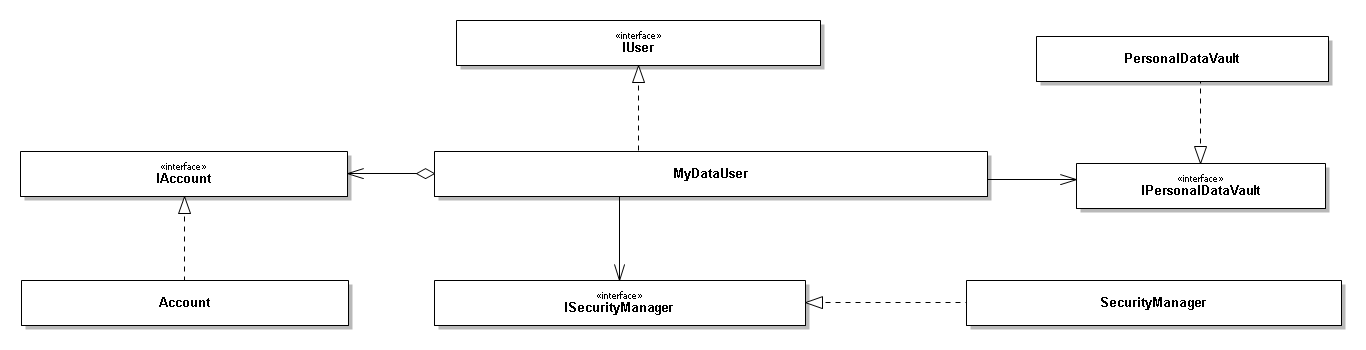
\includegraphics[width=\linewidth]{pictures/Accounting-closed.png}
	\caption{caption}
	\label{fig:Accounting-closed}
\end{figure}
Al centro \`e collocata la classe corrispondente all’utente \textit{MyData}, che, confermando quanto detto in Analisi, \`e collegata agli account dei servizi, e al \texttt{PersonalDataVault} dell’utente. Una novit\`a \`e invece la coppia \texttt{ISecurityManager}, \texttt{SecurityManager} creata per soddisfare i requisiti di sicurezza relativi alla mutua autenticazione fra utente e servizio. Si \`e deciso di sviluppare separatamente questa classe per un principio di separazione delle responsabilit\`a, e per permettere una pi\`u semplice estendibilit\`a in caso di sviluppi futuri.

\subsection{IUser, MyDataUser}
\begin{figure} [h]
	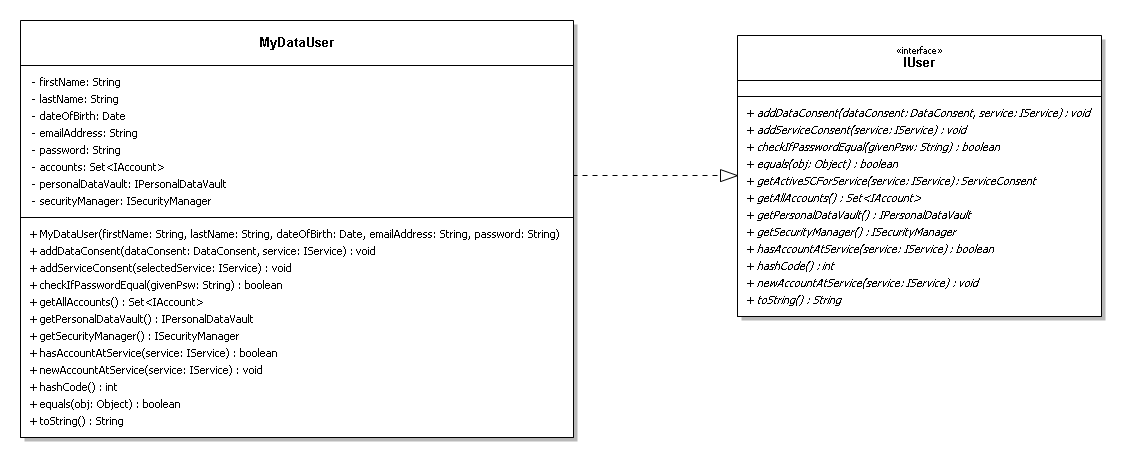
\includegraphics[width=\linewidth]{pictures/Accounting-MyDataUsr.png}
	\caption{caption}
	\label{fig:Accounting-MyDatUsr}
\end{figure}
Questa classe modella un generico utente dell’architettura \textit{MyData}. I field al suo interno sono un esempio delle caratteristiche che si \`e scelto di modellare, e fra di essi i pi\`u rilevanti sono indirizzo email e password, in quanto permettono il login per utenti gi\`a registrati. L’indirizzo mail \`e stato adottato inoltre come identificatore unico di un utente all’interno di \textit{MyData}, e questa caratteristica \`e stata implementata mediante l’override della funzione \texttt{equals(Object obj)}.

Si evidenzia inoltre la presenza di un \texttt{Set<IAccount> accounts}, che realizza l’associazione fra un utente e gli account presso i servizi a cui si \`e registrato. La scelta di un \texttt{Set} permette di implementare il vincolo secondo cui ogni utente pu\`o avere un solo account presso un certo servizio, ed \`e adatta anche in quanto non \`e necessario mantenere un insieme ordinato di account.

Questa classe ha inoltre la funzione di interfacciare gli altri componenti del gestore, compresa la GUI, con gli account utente. A tal fine, presenta i metodi \texttt{addServiceConsent(IService service)}, \texttt{addDataConsent(DataConsent  dataConsent, IService service)}, \texttt{hasAccountAtService(IService service)}.  La classe \texttt{Account} \`e stata infatti modellata con visibilit\`a package protected, per impedire l’accesso a classi esterne al package \texttt{users}: di conseguenza, anche la creazione di nuovi account avviene attraverso questa classe, in particolare nella funzione \texttt{newAccountAtService(IService service)}. All’interno del metodo troviamo l’istanziazione di un nuovo account, insieme ad una chiamata alla classe \texttt{ConsentManager}, che realizza quanto anticipato al paragrafo \ref{sec:A-Consent} a pagina \pageref{sec:A-Consent}. In questo modo si realizza un esempio di \textit{Service Linking}, e l’esito di questa operazione viene concretizzato in un oggetto \texttt{ServiceConsent}. Si rimandano per\`o ulteriori dettagli a quanto spiegato nella sezione \ref{sec:P-AutorizzazioniEConsent} a pagina \pageref{sec:P-AutorizzazioniEConsent}.

\subsection{IAccount, Account}
\begin{figure} [h]
	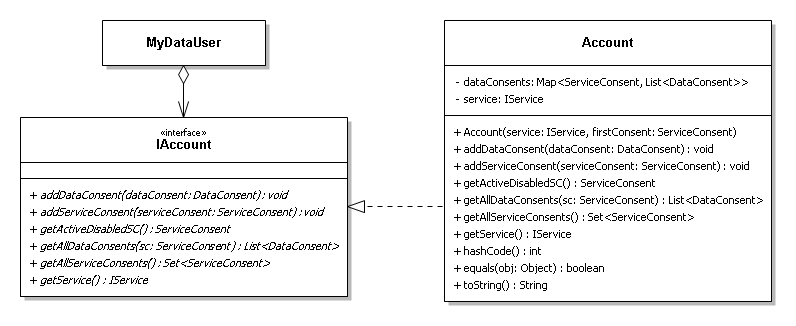
\includegraphics[width=\linewidth]{pictures/Accounting-Account.png}
	\caption{caption}
	\label{fig:Accounting-Account}
\end{figure}
La classe \texttt{Account} \`e abbastanza semplice, poich\'e si occupa semplicemente di implementare la logica di basso livello nelle operazioni di gestione degli account.

Fra queste vi sono i controlli sullo stato dei Consent memorizzati, la gestione dello storico di tutti i Consent emessi per quel servizio service, o ancora il matching fra i due tipi di Consent (\texttt{ServiceConsent}, \texttt{DataConsent}, dettagliati al paragrafo \ref{subsec:P-ServiceConsentDataConsent} a pagina \pageref{subsec:P-ServiceConsentDataConsent}).

La memorizzazione dei Consent all’interno della classe \`e stata ottenuta mediante l’utilizzo combinato delle strutture dati \texttt{Map<ServiceConsent, List<DataConsent>>}. Questa scelta permette di esprimere diversi concetti a livello semantico. Come prima cosa, per i Consent sul flusso di dati si \`e scelto di utilizzare la classe base \texttt{DataConsent} invece che le sue due implementazioni, in modo da poterli memorizzare indiscriminatamente. Ci\`o verifica l’utilizzo del principio di sostituibilit\`a di Liskov. Inoltre, la scelta di una \texttt{List} come value all’interno di una mappa permette di descrivere un flusso di dati (all’interno dello stesso \texttt{ServiceConsent}) per il quale si sono rivelate necessare una molteplicit\`a di interazioni fra \textit{Source} e \textit{Sink}, ognuna delle quali modellata da un \texttt{DataConsent}.

Ad ogni istanza di \texttt{ServiceConsent} corrisponde quindi una \texttt{Collection} dei \texttt{DataConsent} emessi durante il periodo di validit\`a dello stesso, ed \`e possibile avere un unico \texttt{ServiceConsent} attivo in un determinato istante di tempo.

\section{SecurityManager}
\begin{figure} [h]
	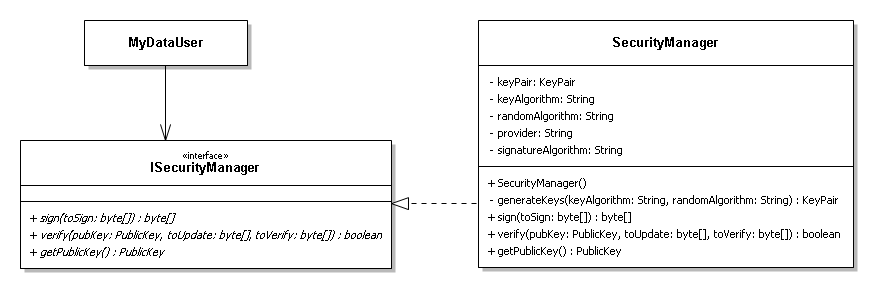
\includegraphics[width=\linewidth]{pictures/Accounting-SecurityManager.png}
	\caption{caption}
	\label{fig:Accounting-SecurityManager}
\end{figure}
https://docs.oracle.com/javase/tutorial/security/TOC.html
http://docs.oracle.com/javase/6/docs/technotes/guides/security/crypto/CryptoSpec.html

\section{IMyData, MyData}
\begin{figure} [h]
	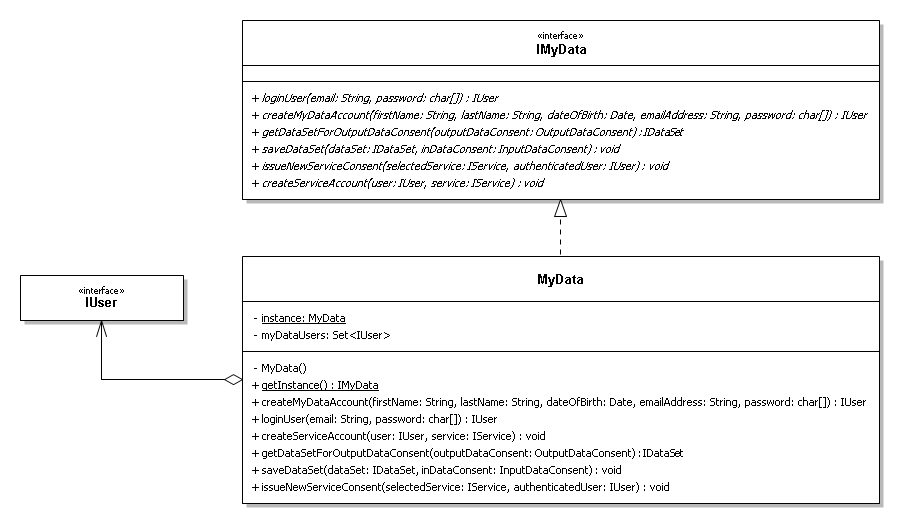
\includegraphics[width=\linewidth]{pictures/MyData.png}
	\caption{caption}
	\label{fig:Accounting-MyData}
\end{figure}

\section{Autorizzazioni e Consent}
\label{sec:P-AutorizzazioniEConsent}
\begin{figure} [h]
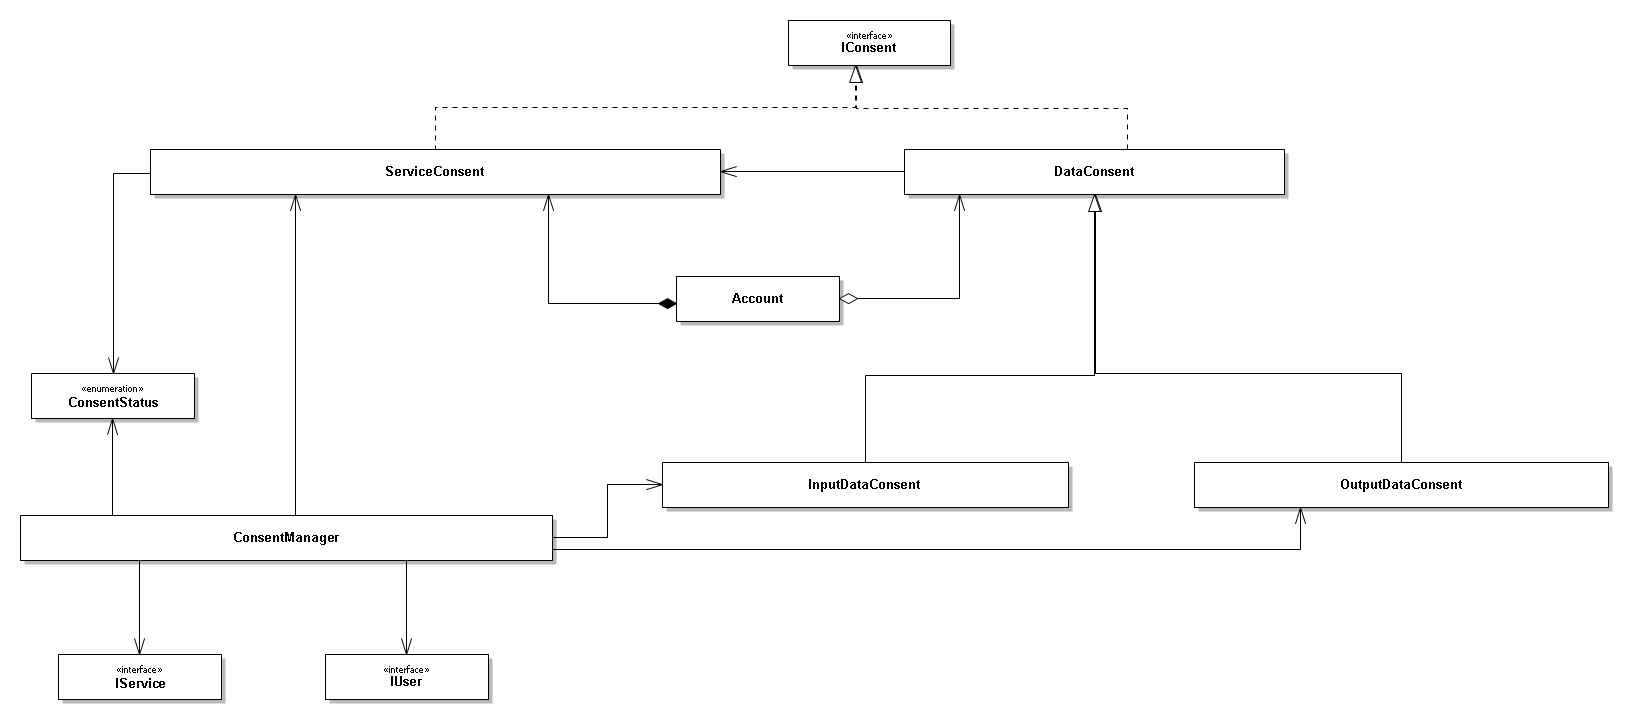
\includegraphics[width=\linewidth]{pictures/Auth-closed.png}
\caption{caption}
\label{fig:Auth-closed}
\end{figure}

\subsection{ConsentManager, ConsentStatus}
\begin{figure} [h]
	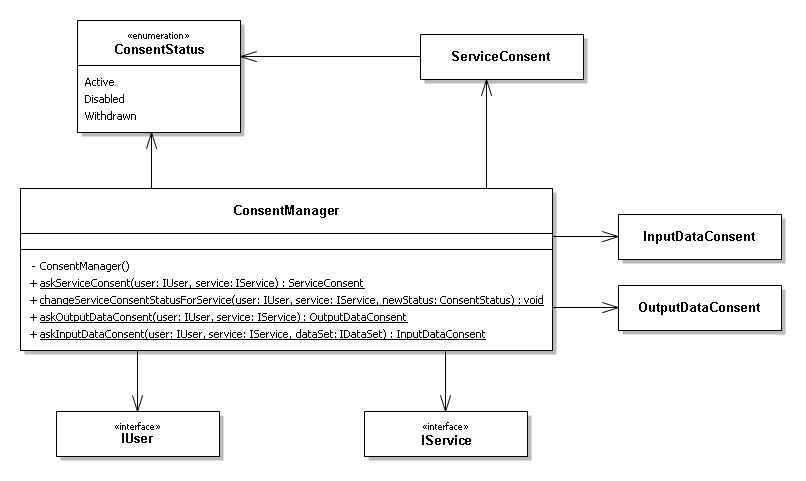
\includegraphics[width=\linewidth]{pictures/Auth-CM.png}
	\caption{caption}
	\label{fig:Auth-CM}
\end{figure}

\subsection{ServiceConsent, DataConsent}
\label{subsec:P-ServiceConsentDataConsent}
\begin{figure} [h]
	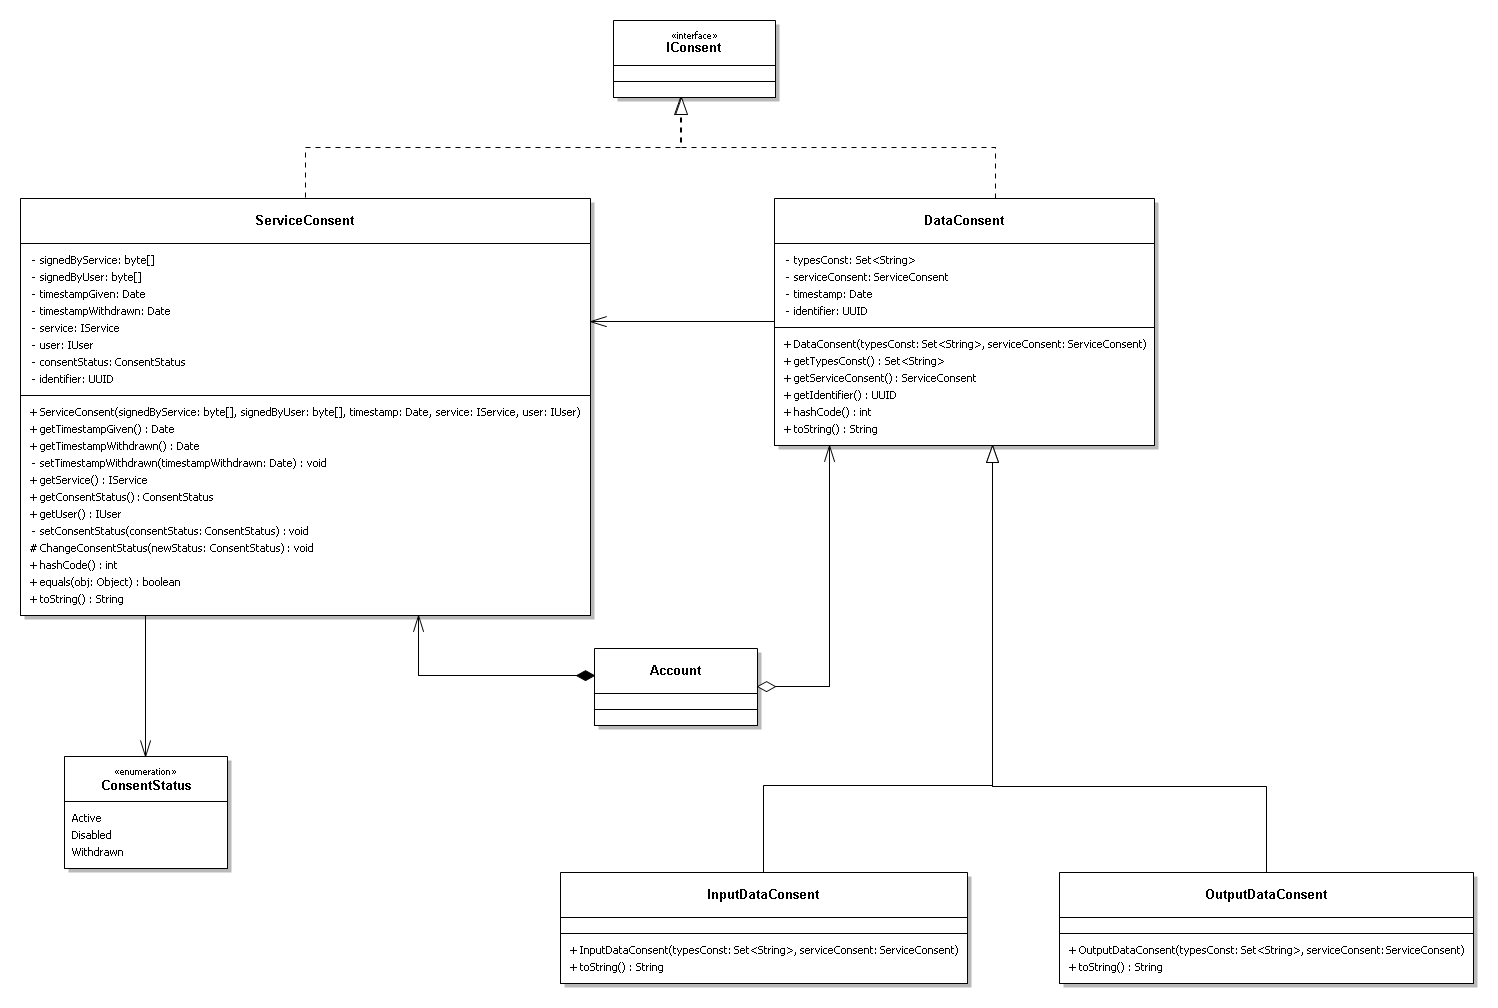
\includegraphics[width=\linewidth]{pictures/Auth-Consents.png}
	\caption{caption}
	\label{fig:Auth-Consents}
\end{figure}
https://docs.oracle.com/javase/8/docs/api/java/security/Permission.html

\section{PersonalDataVault}
\begin{figure} [h]
	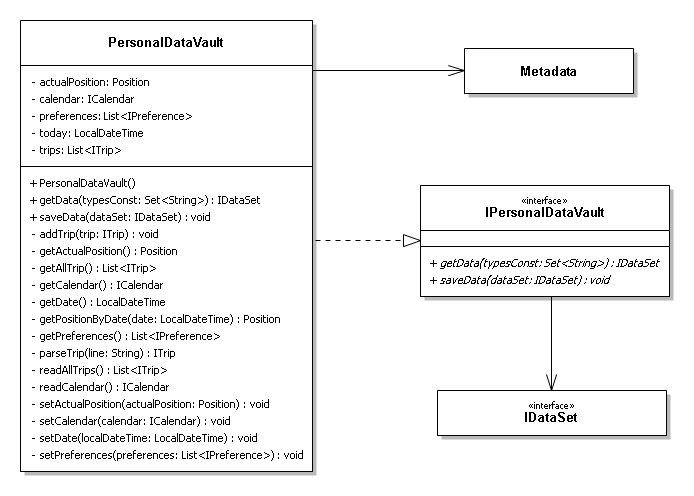
\includegraphics[width=\linewidth]{pictures/PersonalDataVault.png}
	\caption{caption}
	\label{fig:PersonalDataVault}
\end{figure}

\section{Metadata, DataSet}
\begin{figure} [h]
	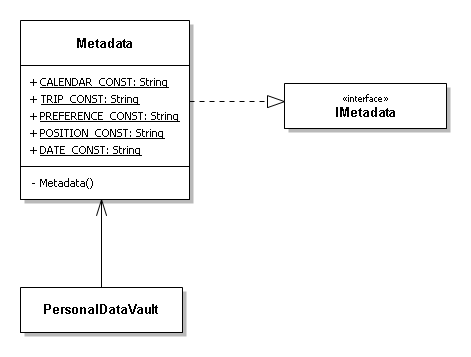
\includegraphics[width=\linewidth]{pictures/Metadata.png}
	\caption{caption}
	\label{fig:Metadata}
\end{figure}

\begin{figure} [h]
	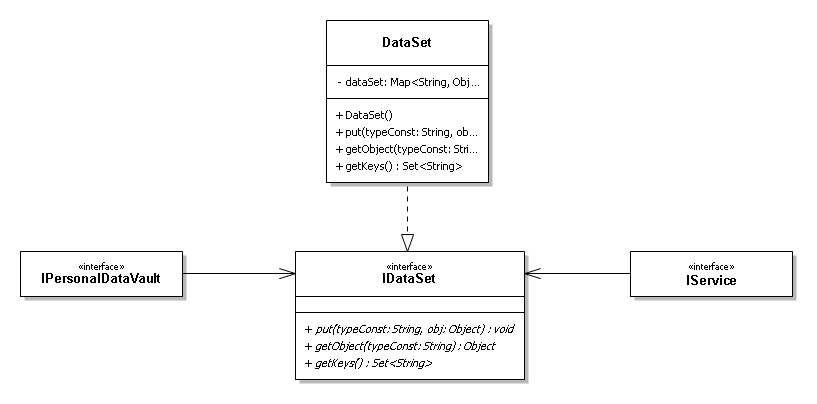
\includegraphics[width=\linewidth]{pictures/IDataSet.png}
	\caption{caption}
	\label{fig:IDataSet}
\end{figure}

\section{IService, AbstractService, MostLikelyNextTrip}
\begin{figure} [h]
	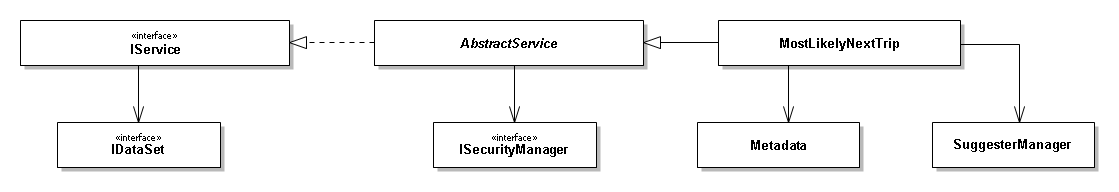
\includegraphics[width=\linewidth]{pictures/Services-closed.png}
	\caption{caption}
	\label{fig:Services-closed}
\end{figure}

\begin{figure} [h]
	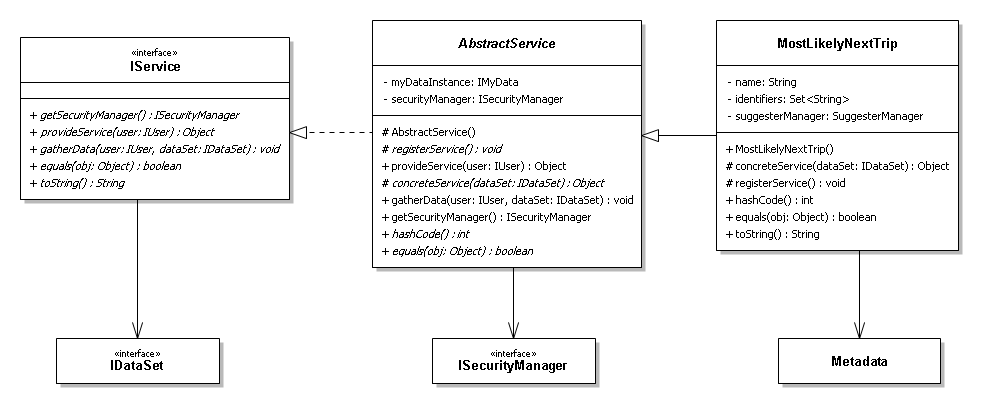
\includegraphics[width=\linewidth]{pictures/Services-open.png}
	\caption{caption}
	\label{fig:Services-open}
\end{figure}

\section{ServiceRegistry}
\begin{figure} [h]
	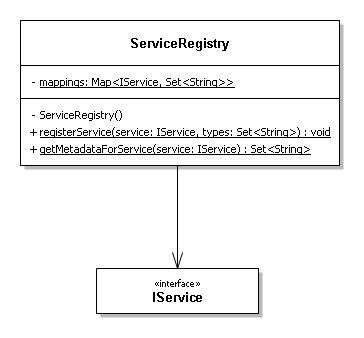
\includegraphics[width=\linewidth]{pictures/ServiceRegistry.png}
	\caption{caption}
	\label{fig:ServiceRegistry}
\end{figure}

\section{Uso delle eccezioni}